\justifying
\chapter{Results}
\label{chapter3}

<Results, evaluation (including user evaluation) {\em etc.} should be described in one or more chapters. See the `Results and Discussion' criterion in the mark scheme for the sorts of material that may be included here.>
\section{Performance}

The table below presents the performance metrics of our FFT-based ocean generation technique on two different GPUs: M1 and Nvidia GeForce RTX 4070. The metrics were recorded for three different texture sizes: 256x256, 512x512, and 1024x1024.

% table for performance
\begin{table}[h]
    \centering
    \begin{tabular}{|c|c|c|}
        \hline
        \textbf{GPU} & \textbf{Texture Size} & \textbf{Time} \\
        \hline
        M1 & 256x256 & 8.56ms \\
        \hline
        M1 & 512x512 & 43.50ms \\
        \hline
        M1 & 1024x1024 & 128.25ms \\
        \hline
        Nvidia GeForce RTX 4070 & 256x256 & 1.65ms \\
        \hline
        Nvidia GeForce RTX 4070 & 512x512 & 3.29ms \\
        \hline
        Nvidia GeForce RTX 4070  & 1024x1024 & 10.70ms \\
        \hline
    \end{tabular}
\end{table}

The data reveals that for a texture size of 256x256, both GPUs are capable of rendering the ocean in real-time, demonstrating the broad applicability of our technique. However, as the texture size increases, the performance on the M1 GPU deteriorates significantly, indicating that our technique becomes computationally expensive for weaker GPUs at higher texture sizes.

Interestingly, the use of cascades in our technique mitigates this issue to an extent. Cascades allow us to maintain a relatively consistent level of detail in the ocean’s visual representation, even when the texture size is increased. This feature makes our technique a viable option for game development across a wide range of computer systems, despite the performance variations observed with different GPUs and texture sizes. Thus, our FFT-based ocean generation technique exhibits a balance between visual fidelity and computational efficiency, making it a promising approach for real-time ocean rendering.

\section{Ablation Study}


\section{Comparison} 

\subsection{Spectrums}
The main diffrence comes to what kind of spectrum you use for FFT based oceans. The proposed "Phillips" spectrum \ref{fig:phillip_spectrum_comp} by \cite[J. Tessendorf]{tessendorf2001} has issues with energy transformation and following the wind direction. 
The proposed TMA spectrum \ref{fig:tma_spectrum_comp} handles energy transformation way more relistic and does not have any issues following the wind direction. This is mostly because that TMA is based on empirical data.
You can see clear diffrence between "Phillips" spectrum and TMA spectrum:

\begin{minipage}{0.48\textwidth}
    \centering
    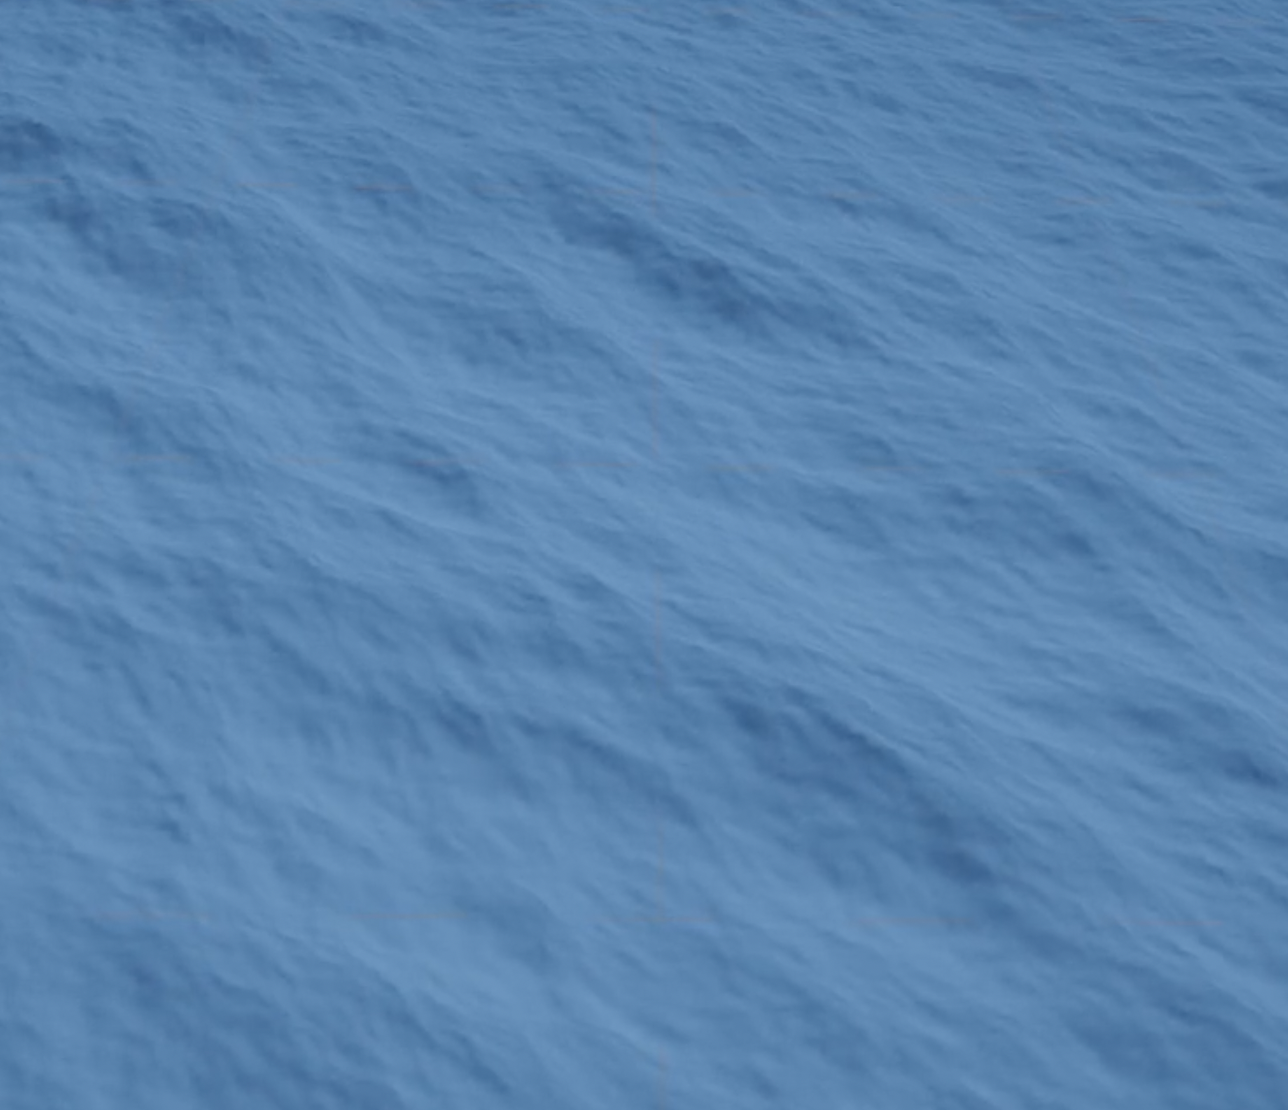
\includegraphics[width=0.8\textwidth]{"images/phillip_spectrum_comp.png"}
    \captionof{figure}{Height Map with $P_h$}
    \label{fig:phillip_spectrum_comp}
\end{minipage}
\hfill
\begin{minipage}{0.48\textwidth}
    \centering
    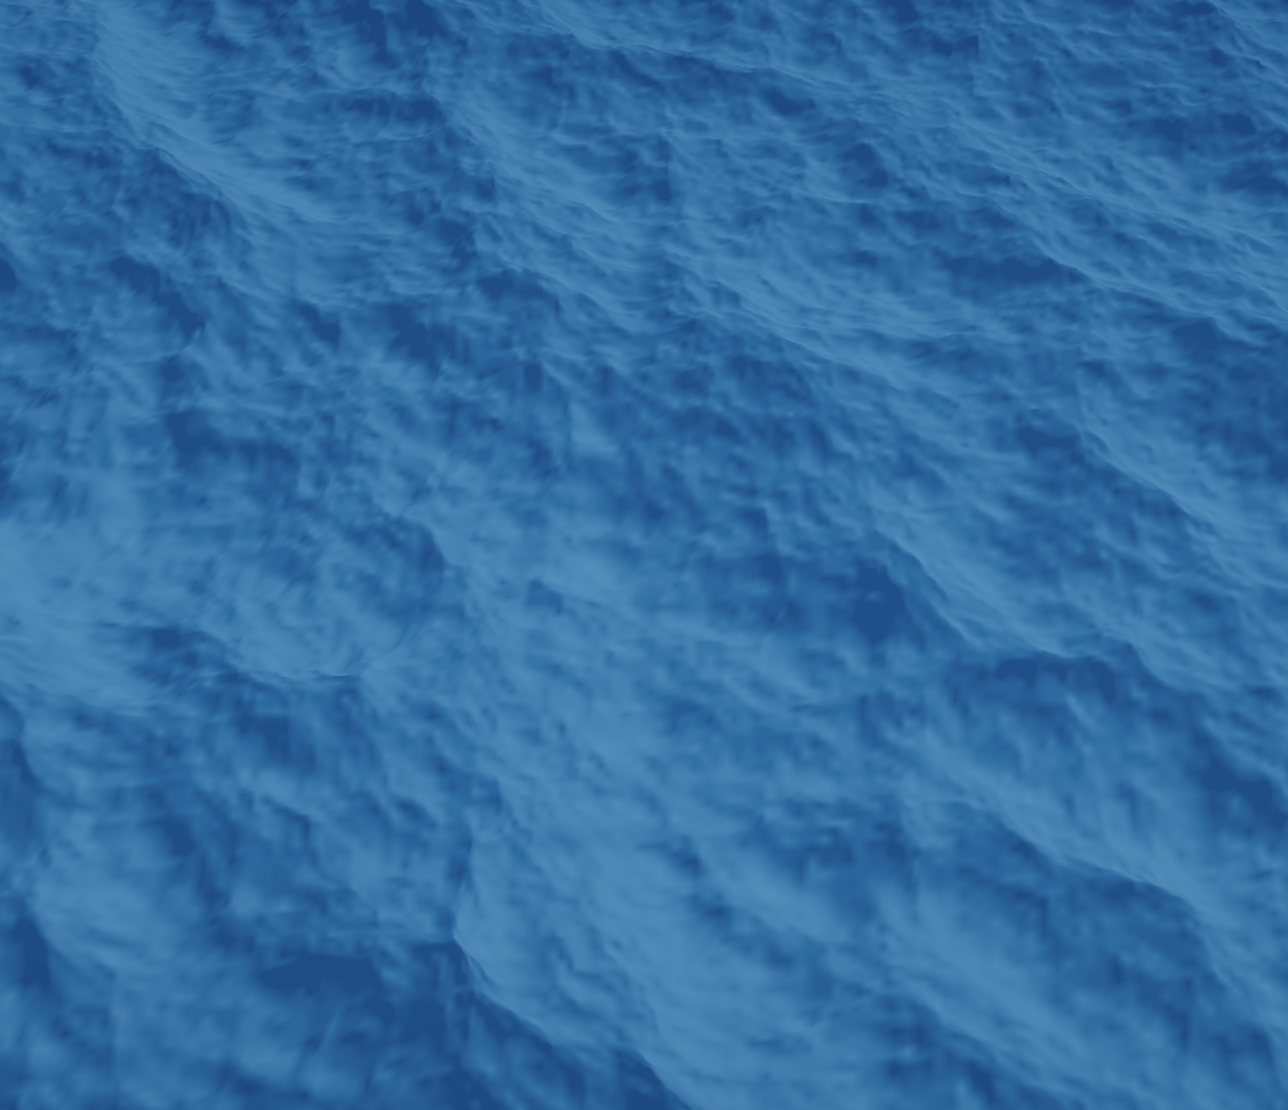
\includegraphics[width=0.8\textwidth]{"images/tma_spectrum_comp.png"}
    \captionof{figure}{Height Map using TMA Spectrum}
    \label{fig:tma_spectrum_comp}
\end{minipage}

\subsection{Real world oceans}
When it comes to calm ocean, the FFT based ocean with TMA spectrum performs extremelly well and holds the desired shape as shown in figures \ref{fig:real_calm_ocean} and \ref{fig:fake_calm_ocean}.
\begin{table}[h]
    \centering
    \begin{tabular}{|c|c|c|c|c|c|c|c|c|c|}
        \hline
        \textbf{Spectrum} & \textbf{Size} & $\mathbf{l_1}$ & $\mathbf{l_2}$ & $\mathbf{l_3}$ & $\mathbf{\lambda}$ & $\mathbf{U_{10}}$ & \textbf{Fetch} & \textbf{Depth} \\
        \hline
        256x256 & TMA & 256 & 100 & 10 & 0.9 & 0.5 m/s & 1000 km & 500 m \\
        \hline
    \end{tabular}
    \caption{Calm Ocean Parameters}
    \label{tab:calm_ocean}
\end{table}

\begin{minipage}{0.48\textwidth}
    \centering
    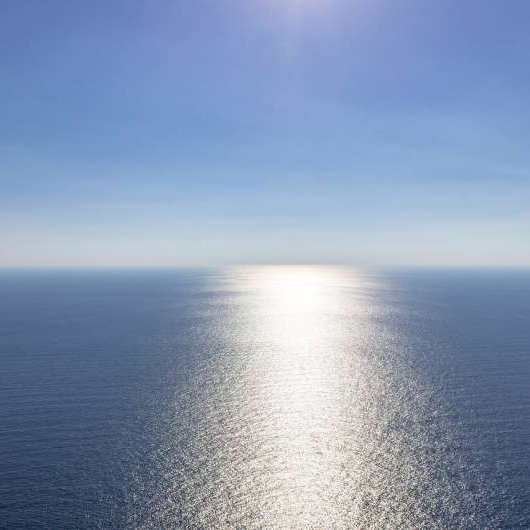
\includegraphics[width=1\textwidth]{"images/real_calm_ocean.jpg"}
    \captionsetup{justification=centering}
    \captionof{figure}{Calm Atlantic Ocean\\ Credits: CC0 Public Domain}
    \label{fig:real_calm_ocean}
\end{minipage}
\hfill
\begin{minipage}{0.48\textwidth}
    \centering
    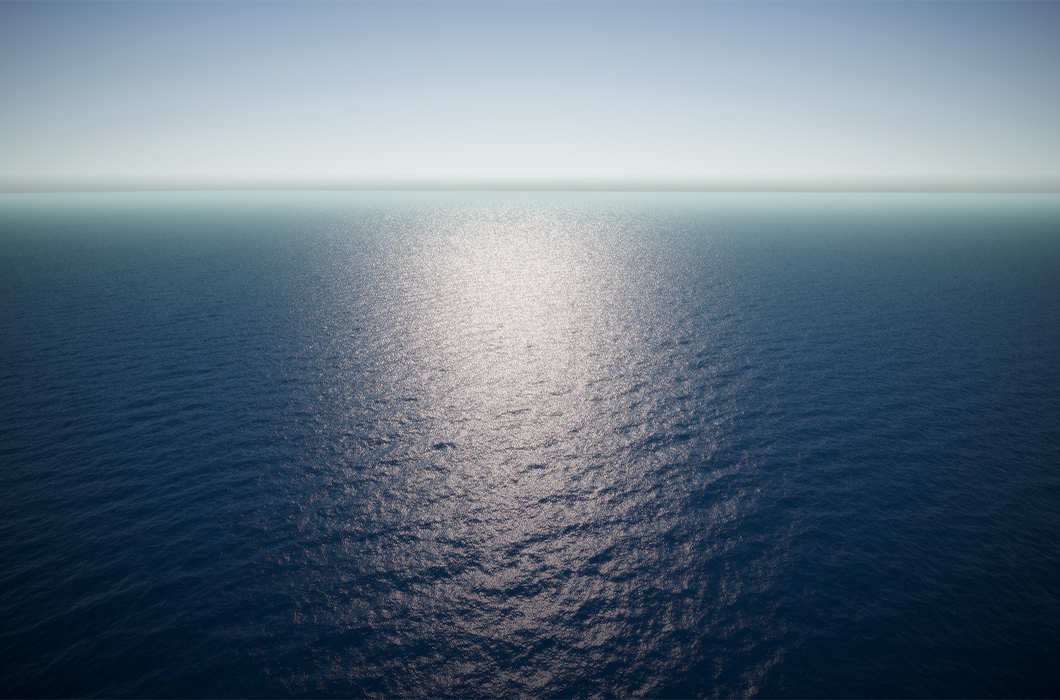
\includegraphics[width=1\textwidth]{"images/fake_calm_ocean.png"}
    \captionof{figure}{FFT Calm \\ Ocean}
    \label{fig:fake_calm_ocean}
\end{minipage}

When it comes to stormy ocean where huge waves is expected the general shape of an ocean is still relistic
and can hadle the big waves without any trouble, and because of diffrent cascades the tilling is bearlly noticible as shown in the following figures \ref{fig:real_stormy_ocean} and \ref{fig:fake_stormy_ocean}.

\begin{table}[h]
    \centering
    \begin{tabular}{|c|c|c|c|c|c|c|c|c|c|}
        \hline
        \textbf{Spectrum} & \textbf{Size} & $\mathbf{l_1}$ & $\mathbf{l_2}$ & $\mathbf{l_3}$ & $\mathbf{\lambda}$ & $\mathbf{U_{10}}$ & \textbf{Fetch} & \textbf{Depth} \\
        \hline
        256x256 & TMA & 700 & 256 & 70 & 0.9 & 21 m/s & 1000 km & 500 m \\
        \hline
    \end{tabular}
    \caption{Stormy Ocean Parameters}
    \label{tab:stormy_ocean}
\end{table}

where each $l$ is the wave length scale of each cascade.

\begin{minipage}{0.48\textwidth}
    \centering
    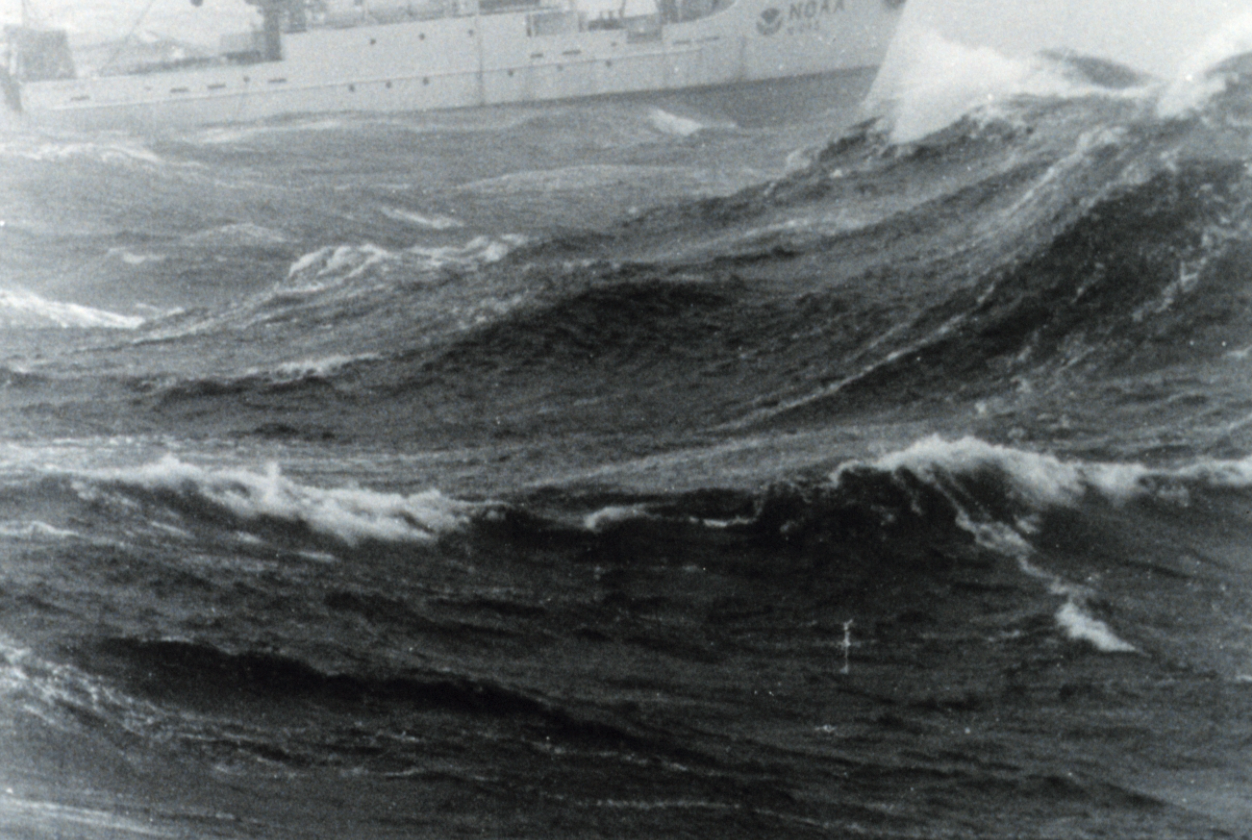
\includegraphics[width=1\textwidth]{"images/real_stormy_ocean.png"}
    \captionsetup{justification=centering}
    \captionof{figure}{Calm Atlantic Ocean\\ Credits: CC0 Public Domain}
    \label{fig:real_stormy_ocean}
\end{minipage}
\hfill
\begin{minipage}{0.48\textwidth}
    \centering
    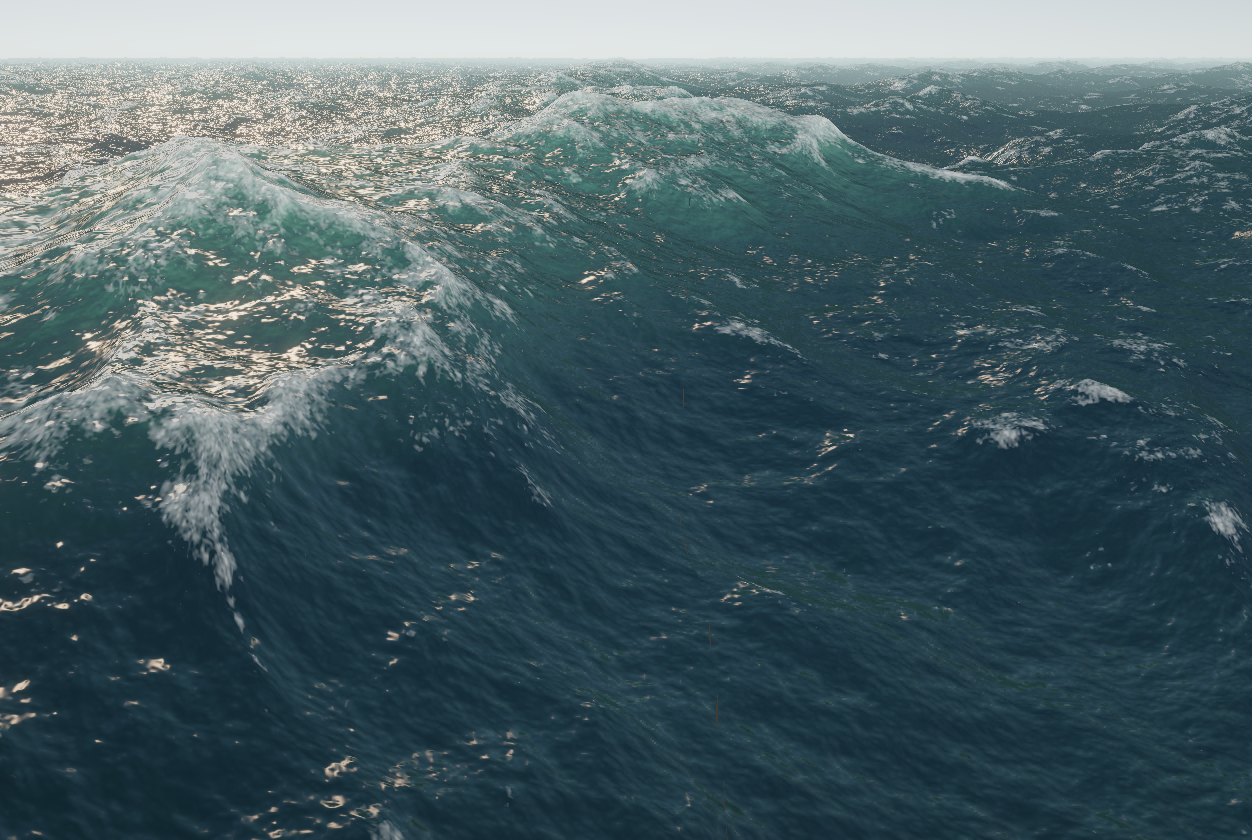
\includegraphics[width=1\textwidth]{"images/fake_stormy_ocean.png"}
    \captionof{figure}{Height Map using\\ TMA Spectrum}
    \label{fig:fake_stormy_ocean}
\end{minipage}

\section{Diffrent Outputs}

\begin{minipage}{1\textwidth}
    \centering
    \includegraphics[width=1\textwidth]{"images/output1.png"}
    \captionof{figure}{Calm ocean with blue sky}
    \label{fig:output_1}
\end{minipage}

\begin{table}[h]
    \centering
    \begin{tabular}{|c|c|c|c|c|c|c|c|c|c|}
        \hline
        \textbf{Spectrum} & \textbf{Size} & $\mathbf{l_1}$ & $\mathbf{l_2}$ & $\mathbf{l_3}$ & $\mathbf{\lambda}$ & $\mathbf{U_{10}}$ & \textbf{Fetch} & \textbf{Depth} \\
        \hline
        256x256 & TMA & 400 & 100 & 10 & 2 & 0.5 m/s & 1000 km & 500 m \\
        \hline
    \end{tabular}
    \caption{Calm Ocean Parameters}
    \label{tab:output_1}
\end{table}

\begin{minipage}{1\textwidth}
    \centering
    \includegraphics[width=1\textwidth]{"images/output2.png"}
    \captionof{figure}{Stormy Ocean with cloudy enviroment}
    \label{fig:output_2}
\end{minipage}

\begin{table}[h]
    \centering
    \begin{tabular}{|c|c|c|c|c|c|c|c|c|c|}
        \hline
        \textbf{Spectrum} & \textbf{Size} & $\mathbf{l_1}$ & $\mathbf{l_2}$ & $\mathbf{l_3}$ & $\mathbf{\lambda}$ & $\mathbf{U_{10}}$ & \textbf{Fetch} & \textbf{Depth} \\
        \hline
        256x256 & TMA & 800 & 256 & 10 & 0.95 & 31 m/s & 1000 km & 500 m \\
        \hline
    \end{tabular}
    \caption{Stormy Ocean Parameters}
    \label{tab:output_2}
\end{table}

\begin{minipage}{1\textwidth}
    \centering
    \includegraphics[width=1\textwidth]{"images/output3.png"}
    \captionof{figure}{Ocean with Medium Waves}
    \label{fig:output_3}
\end{minipage}

\begin{table}[h]
    \centering
    \begin{tabular}{|c|c|c|c|c|c|c|c|c|c|}
        \hline
        \textbf{Spectrum} & \textbf{Size} & $\mathbf{l_1}$ & $\mathbf{l_2}$ & $\mathbf{l_3}$ & $\mathbf{\lambda}$ & $\mathbf{U_{10}}$ & \textbf{Fetch} & \textbf{Depth} \\
        \hline
        256x256 & TMA & 600 & 256 & 10 & 1.3 & 12 m/s & 1000 km & 500 m \\
        \hline
    \end{tabular}
    \caption{Medium Waves Parameters}
    \label{tab:output_1}
\end{table}

\section{Known Problems}
During the implementation of our FFT-based ocean generation technique, we encountered challenges related to the global application of FFT-generated maps. This global application restricts us from selectively altering specific sections of the sea, such as the wake created by a moving ship or the reduced wave height near a shallow beach.

To address these challenges, J. Tessendorf proposed a hybrid approach in his paper \cite{tessendorf2004}. This approach combines grid-based ocean generation, where each vertex point is propagated individually and FFT waves serve as ambient waves. Tessendorf later enhanced this approach with the release of “eWaves” \cite{tessendorf2014}.

These challenges underscore the complexities involved in ocean wave simulation and the potential of hybrid approaches in advancing the field. The proposed hybrid approach effectively addresses the identified challenges, demonstrating its potential in enhancing the realism and interactivity of ocean wave simulations.


